% RESULTADOS-------------------------------------------------------------------

\chapter{Análise e Discussão dos Resultados}
\label{chap:resultados}

Este capítulo discute os resultados obtidos nas duas abordagens de esteganálise estudadas neste trabalho. Como descrito anteriormente, a primeira é baseada no descritor SRM - posteriormente utilizado em um conjunto (\textit{ensemble}) de classificadores - e a segunda em CNNs. 

Conforme detalhado no capítulo anterior, são considerados 12 conjuntos de treinamento, resultantes da aplicação dos algoritmos de esteganografia HUGO, S-UNIWARD e MiPOD para quatro diferentes \textit{payloads}: 0.1, 0.2, 0.4 e 0.6 bpp. Visando facilitar a identificação de um conjunto específico, serão consideradas as siglas definidas na Tabela~\ref{tab:cenariosTrain}, compostas pela primeira letra do nome do algoritmo de esteganografia seguida do valor do \textit{payload} (por exemplo, H6 representa HUGO com \textit{payload} 0.6 bpp).

Além disso, também são definidos 28 conjuntos de teste, listados na Tabela~\ref{tab:cenariosTest}. Cada um deles é identificado por uma sigla composta pela primeira letra do nome do algoritmo de esteganografia utilizado para gerar a estego imagem, seguida por dois valores: um  que representa o STC e outro que identifica o \textit{payload} (por exemplo, H.0.2 representa o HUGO com STC 0 e \textit{payload} 0.2 bpp).

Cada um dos 12 conjuntos de treinamento é utilizado separadamente para treinamento das duas abordagens de esteganálise. Os modelos de classificação resultantes (\textit{ensemble} de classificadores ou CNN) são então aplicados em diferentes conjuntos de teste (x denota a variação para os quatro \textit{payloads}):
\begin{enumerate}%TODO
\item SRM + \textit{Ensemble}: sete conjuntos - H.0.x, H.10.x, S.0.x, S.10.1, S.10.4, S.10.6, M.0.x\footnote{Por limitação de tempo não foram realizados os demais testes.}.
\item CNN: todos os 28 conjuntos listados na Tabela~\ref{tab:cenariosTest} - H.0.x, H.10.x, S.0.x, S.7.x, S.10.x, S.12.x, M.-.x.
\end{enumerate}
Com isso, tem-se um total de 12 $\times$ 7 + 12 $\times$ 28 = 420 resultados.

Na sequência, serão discutidos os resultados obtidos, os quais serão divididos por abordagem de esteganálise e depois por conjunto de treinamento. Ao final, será realizada uma análise geral dos resultados. Os Apêndices \ref{chap:apendiceA} e \ref{chap:apendiceB} mostram tabelas das áreas sob a curva (AUC) obtidas nos testes com SRM e CNN respectivamente.

\clearpage
\section{Resultados com SRM e \textit{Ensemble} de Classificadores}

Em geral, o comportamento da seleção de características é semelhante para todos \textit{payloads}de 1000 à 1400 características. No caso do número de classificadores, os dois \textit{payloads} menores variam de 70 à 80 enquanto os maiores variam de 90 à 100. Tais comportamentos são ilustrado na Figura \ref{fig:srm_train}, para o caso do conjunto de treinamento M1.

\begin{figure}[ht]
\centering
	\subfloat[]{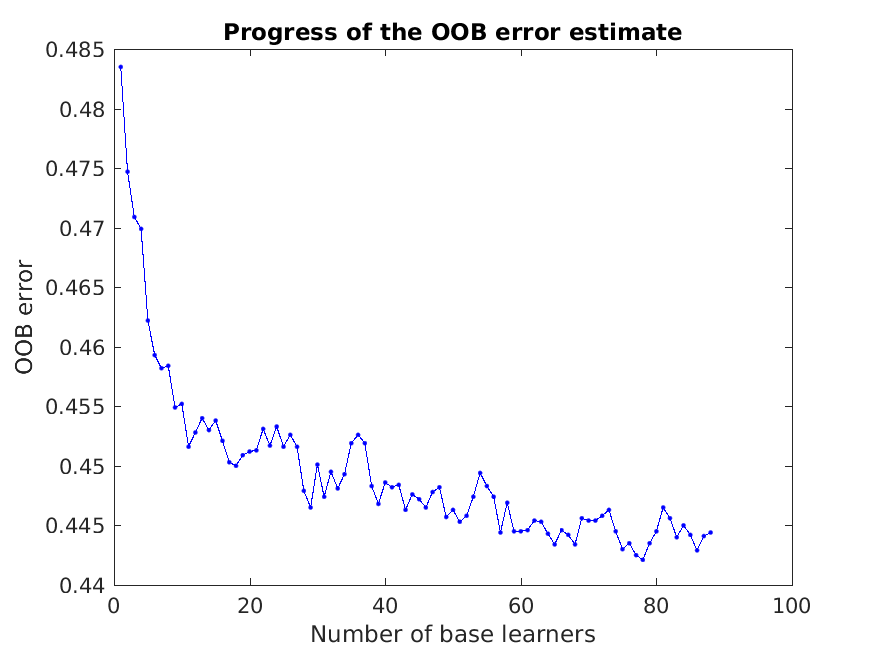
\includegraphics[width=0.7\textwidth]{dados/figuras/oob.png}}\qquad
	\subfloat[]{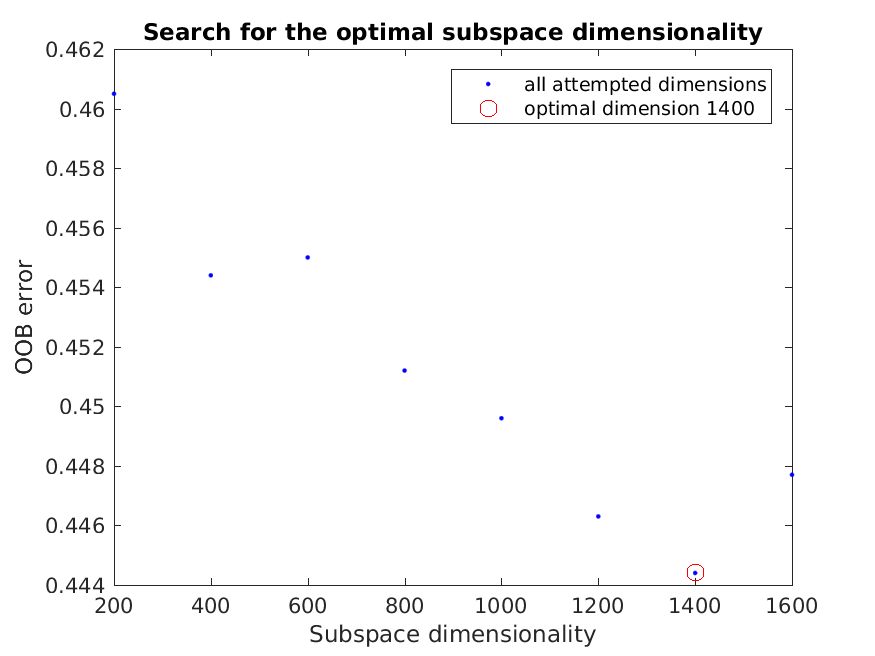
\includegraphics[width=0.7\textwidth]{dados/figuras/dimesion.png}}\\ 

\caption{(a) Variação do OOBe com relação ao número de classificadores para o cojunto de treinamento M1. (b) Variação do OOBe com relação ao número de características para o conjunto de treinamento M1 (Autoria própria).}
\label{fig:srm_train}
\end{figure}

Outro fato interessante é o comportamento dos classificadores base para os diferentes \textit{payloads} de teste. A Figura \ref{fig:votes}(a) mostra a assertividade quando o \textit{payload} de treinamento e teste são próximos, dado que existe uma tendência do indicador estar próximo da extremidade e com os tipos de imagens, estego ou cobertura, na posição desejada.

Além disso, quando o classificador treinado em um conjunto de treinamento com  \textit{payload} alto é aplicado em um conjunto de testes que possui \textit{payload} baixo, o histograma tende a estar mais elevado para a esquerda tanto para as imagens de cobertura quanto para as estego imagens. Isso ocorre porque, como o \textit{payload} de teste é muito menor que o de treino, a rede confunde quase todas as imagens com imagens de cobertura. Esse comportamento é recíproco para \textit{payloads} de treino e teste inversos, porém a confusão ocorre com estego imagens (um exemplo pode ser visto na Figura \ref{fig:votes}(b)).

\begin{figure}[!htb]
\centering
	\subfloat[]{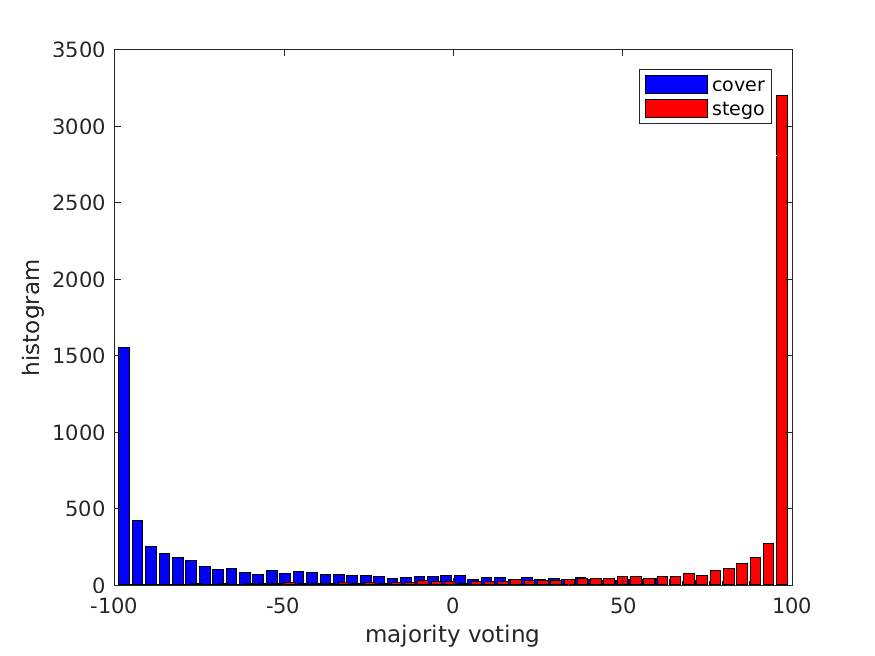
\includegraphics[width=0.45\textwidth]{dados/figuras/voting2.png}}\qquad
	\subfloat[]{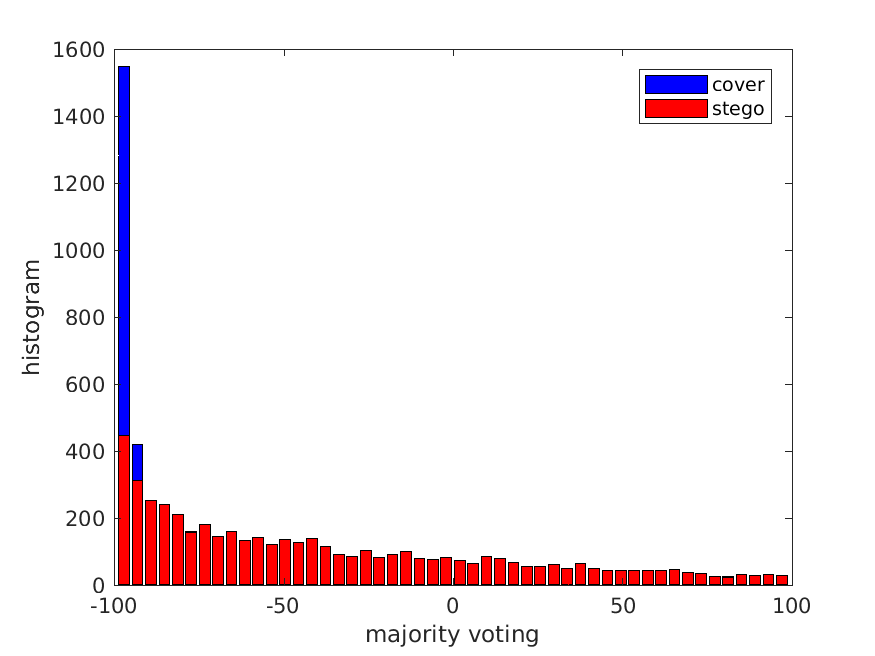
\includegraphics[width=0.45\textwidth]{dados/figuras/voting3.png}}\\ 

\caption{(a) Histograma de votação para o conjunto de treino H4 e de teste H.0.6. (b) Histograma de votação para o conjunto de treino H6 e de teste H.0.1. (Autoria própria)}
\label{fig:votes}
\end{figure}





As seções a seguir apresentarão os resultados da classificação das imagens com o uso do descritor SRM para os 12 diferentes conjuntos de treino.

\clearpage
\subsection{Conjunto de Treinamento H1}

Os resultados para o conjunto de treinamento H1 podem ser vistos na Tabela \ref{tab:srm_h1}. Os melhores resultados foram obtidos com o \textit{payload} de teste igual ao de treino e resultados inferiores nos demais cenários de teste. Essas situações mostram as principais características observadas ao se usar o descritor SRM com \textit{ensemble} de classificadores: melhores performances quando se usando \textit{payload} próximo e mesmo algoritmo de treino e teste, baixa performance ao testar com \textit{payloads} muito distintos do de teste, além da facilidade na detecção do algoritmo HUGO em relação aos outros dois algoritmos.

\begin{table}[!htb]
\centering
\begin{tabular}{c|c|c|c|c|}
\cline{2-5}
\textbf{}                             & \textbf{x = 0.1} & \textbf{x = 0.2} & \textbf{x = 0.4} & \textbf{x = 0.6} \\ \hline
\multicolumn{1}{|c|}{\textbf{H.0.x}}  & 66,23\%          & 72,48\%          & 77,57\%          & 79,31\%          \\ \hline
\multicolumn{1}{|c|}{\textbf{H.10.x}} & \textbf{67,02\%} & \textbf{73,25\%} & \textbf{77,79\%} & \textbf{79,42\%} \\ \hline
\multicolumn{1}{|c|}{\textbf{S.0.x}}  & 58,78\%          & 66,91\%          & 74,68\%          & 78,11\%          \\ \hline
\multicolumn{1}{|c|}{\textbf{S.10.x}} & 59,78\%          & 67,71\%         & 75,20\%          & 78,24\%          \\ \hline
\multicolumn{1}{|c|}{\textbf{M.-.x}}  & 57,86\%          & 64,77\%          & 71,92\%          & 75,61\%          \\ \hline
\end{tabular}
\caption{Acurácias dos testes do SRM com o conjunto de treinamento H1.}
\label{tab:srm_h1}
\end{table}


\subsection{Conjunto de Treinamento H2}

Do mesmo modo que para o conjunto de treino anterior, os melhores resultados foram obtidos para os cenários de teste com uso do HUGO. Porém, os resultados para os conjuntos H.0.4, H.0.6, H.10.4, H.10.6 foram muito superiores. Os resultados podem ser vistos na Tabela \ref{tab:srm_h2}.

\begin{table}[!htb]
\centering
\begin{tabular}{c|c|c|c|c|}
\cline{2-5}
\textbf{}                             & \textbf{x = 0.1} & \textbf{x = 0.2} & \textbf{x = 0.4} & \textbf{x = 0.6} \\ \hline
\multicolumn{1}{|c|}{\textbf{H.0.x}}  & 63,24\%          & 73,89\%    & 82,23\%          & 84,47\%          \\ \hline
\multicolumn{1}{|c|}{\textbf{H.10.x}} & \textbf{65,03\%} & \textbf{75,30\%} & \textbf{82,70\%} & \textbf{84,69\%} \\ \hline
\multicolumn{1}{|c|}{\textbf{S.0.x}}  & 52,83\%          & 64,02\%          & 77,11\%          & 82,51\%          \\ \hline
\multicolumn{1}{|c|}{\textbf{S.10.x}} & 53,95\%          & 65,86\%          & 78,22\%          & 82,89\%          \\ \hline
\multicolumn{1}{|c|}{\textbf{M.-.x}}  & 52,70\%          & 61,50\%          & 73,73\%          & 79,95\%          \\ \hline
\end{tabular}
\caption{Acurácias dos testes do SRM com o conjunto de treinamento H2.}
\label{tab:srm_h2}
\end{table}


\subsection{Conjunto de Treinamento H4}

A Tabela \ref{tab:srm_h4} mostra que o conjunto apresentou, como esperado, os melhores resultados para o algoritmo HUGO com o \textit{payload} de 0.4 bpp e valores acima de 89\% para os cenários H.10.6 e H.0.6, os quais só não superaram o conjunto de treino H6.

\begin{table}[!htb]
\centering
\begin{tabular}{c|c|c|c|c|}
\cline{2-5}
\textbf{}                             & \textbf{x = 0.1} & \textbf{x = 0.2} & \textbf{x = 0.4} & \textbf{x = 0.6} \\ \hline
\multicolumn{1}{|c|}{\textbf{H.0.x}}  & 53,55\%          & 60,80\%          & 84,60\%          & 89,11\%          \\ \hline
\multicolumn{1}{|c|}{\textbf{H.10.x}} & \textbf{54,85\%} & \textbf{70,39\%} & \textbf{85,43\%} & \textbf{89,36\%} \\ \hline
\multicolumn{1}{|c|}{\textbf{S.0.x}}  & 50,75\%          & 53,75\%          & 73,42\%          & 84,48\%          \\ \hline
\multicolumn{1}{|c|}{\textbf{S.10.x}} & 51,04\%          & 55,46\%         & 75,67\%          & 85,36\%          \\ \hline
\multicolumn{1}{|c|}{\textbf{M.-.x}}  & 50,78\%          & 52,90\%          & 68,50\%          & 80,17\%          \\ \hline
\end{tabular}
\caption{Acurácias dos testes do SRM com o conjunto de treinamento H4}
\label{tab:srm_h4}
\end{table}


\subsection{Conjunto de Treinamento H6}

Nos experimentos, o conjunto de treinamento H6 obteve os melhores resultados para os cenários H.10.6 e H.0.6 com 91,81\% e 90,46\% de acurácia respectivamente. Os resultados podem ser vistos na Tabela~\ref{tab:srm_h6}.

\begin{table}[!htb]
\centering
\begin{tabular}{c|c|c|c|c|}
\cline{2-5}
\textbf{}                             & \textbf{x = 0.1} & \textbf{x = 0.2} & \textbf{x = 0.4} & \textbf{x = 0.6} \\ \hline
\multicolumn{1}{|c|}{\textbf{H.0.x}}  & 51,13\%          & 58,98\%          & \textbf{81,30\%}          & 90,46\%          \\ \hline
\multicolumn{1}{|c|}{\textbf{H.10.x}} & \textbf{51,46\%} & \textbf{61,14\%} & 77,79\% & \textbf{91,18\%} \\ \hline
\multicolumn{1}{|c|}{\textbf{S.0.x}}  & 50,41\%          & 51,64\%          & 64,44\%          & 79,46\%          \\ \hline
\multicolumn{1}{|c|}{\textbf{S.10.x}} & 50,46\%          & 51,94\%         & 66,66\%          & 81,52\%          \\ \hline
\multicolumn{1}{|c|}{\textbf{M.-.x}}  & 50,38\%          & 51,28\%          & 60,05\%          & 73,73\%          \\ \hline
\end{tabular}
\caption{Acurácias dos testes do SRM com o conjunto de treinamento H6.}
\label{tab:srm_h6}
\end{table}


\subsection{Conjunto de Treinamento S1}

Todos os melhores resultados para o algoritmo S-UNIWARD foram obtidos com os conjuntos treinados com o mesmo algoritmo e mesmo \textit{payload}. No caso do S1, a Tabela \ref{tab:suni_s1} mostra que foram obtidas acurácias interessantes para os cenários H.0.1, H.10.1, S.0.1, S.10.1 e M.1, mesmo que com acurácia muito abaixo da obtida pelos conjuntos treinados e testados com o HUGO para o mesmo \textit{payload}.

\begin{table}[!htb]
\centering
\begin{tabular}{c|c|c|c|c|}
\cline{2-5}
\textbf{}                             & \textbf{x = 0.1} & \textbf{x = 0.2} & \textbf{x = 0.4} & \textbf{x = 0.6} \\ \hline
\multicolumn{1}{|c|}{\textbf{H.0.x}}  & 59,54\%          & 66,68\%          & 74,59\%          & 79,54\%          \\ \hline
\multicolumn{1}{|c|}{\textbf{H.10.x}} & 61,19\%          & 66,43\%          & 75,22\%          & 78,76\%   \\ \hline
\multicolumn{1}{|c|}{\textbf{S.0.x}}  & \textbf{61,53\%}          & \textbf{69,97\%}          & 77,10\%          & \textbf{79,87\%}          \\ \hline
\multicolumn{1}{|c|}{\textbf{S.10.x}} &
61,09\% & 69,75\% & \textbf{77,46\%} & 80,22\% \\ \hline
\multicolumn{1}{|c|}{\textbf{M.-.x}}  & 59,85\%          & 66,06\%          & 73,50\%          & 77,28\%          \\ \hline
\end{tabular}
\caption{Acurácias dos testes do SRM com o conjunto de treinamento S1.}
\label{tab:suni_s1}

\end{table}



\subsection{Conjunto de Treinamento S2}

A Tabela \ref{tab:suni_s2} apresenta os resultados para o conjunto de treino S2. Como já dito anteriormente, o conjunto obteve os melhores resultados para o cenário S.0.2, além de resultados bons para o \textit{payload} de 0.4 bpp.
\begin{table}[!htb]
\centering
\begin{tabular}{c|c|c|c|c|}
\cline{2-5}
\textbf{}                             & \textbf{x = 0.1} & \textbf{x = 0.2} & \textbf{x = 0.4} & \textbf{x = 0.6} \\ \hline
\multicolumn{1}{|c|}{\textbf{H.0.x}}  & 58,65\%          & 69,30\%          & 79,94\%          & 84,37\%          \\ \hline
\multicolumn{1}{|c|}{\textbf{H.10.x}} & 59,67\% & 69,50\% & 79,63\% & 83,82\% \\ \hline
\multicolumn{1}{|c|}{\textbf{S.0.x}}  & 59,20\%          & \textbf{70,40\%}          & 81,24\%         & \textbf{84,90\%}          \\ \hline
\multicolumn{1}{|c|}{\textbf{S.10.x}} & \textbf{60,59\%}          & 71,49\%
& \textbf{82,01\%}          & 84,99\%          \\ \hline
\multicolumn{1}{|c|}{\textbf{M.-.x}}  & 57,60\%          & 66,79\%          & 76,84\%          & 82,05\%          \\ \hline
\end{tabular}
\caption{Acurácias dos testes do SRM com o conjunto de treinamento S2.}
\label{tab:suni_s2}

\end{table}



\subsection{Conjunto de Treinamento S4}

A única exceção a regra, o conjunto S4 obteve tanto os melhores resultados dentre todos os conjuntos de treino tanto para o cenário S.0.4 quanto para o S.0.6. Seus resultados podem ser vistos na Tabela \ref{tab:suni_s4}.

\begin{table}[!htb]
\centering
\begin{tabular}{c|c|c|c|c|}
\cline{2-5}
\textbf{}                             & \textbf{x = 0.1} & \textbf{x = 0.2} & \textbf{x = 0.4} & \textbf{x = 0.6} \\ \hline
\multicolumn{1}{|c|}{\textbf{H.0.x}}  & 53,98\%          & 65,23\%          & 79,86\%          & 88,17\%          \\ \hline
\multicolumn{1}{|c|}{\textbf{H.10.x}} & \textbf{55,33\%} & \textbf{66,08\%} & 81,29\% & 87,86\% \\ \hline
\multicolumn{1}{|c|}{\textbf{S.0.x}}  & 52,81\%          & 64,08\%          & 81,89\%          & \textbf{89,64\%}          \\ \hline
\multicolumn{1}{|c|}{\textbf{S.10.x}} & 53,68\%          & 66,31\%          & \textbf{83,31}\%          & 88,95\%          \\ \hline
\multicolumn{1}{|c|}{\textbf{M.-.x}}  & 52,42\%          & 61,86\%          & 77,99\%          & 85,34\%          \\ \hline
\end{tabular}
\caption{Acurácias dos testes do SRM com o conjunto de treinamento S4.}
\label{tab:suni_s4}

\end{table}

Em comparação ao conjunto S2, os resultados para o \textit{payload} 0.1 foram significativamente melhores, enquanto que o desempenho para o \textit{payload} 0.6 aumentou. Isso sugere que a capacidade do classificador ao ser treinado com 0.4 o torna mais robusto a maiores alterações na imagem, mas prejudica os casos em que há pouca alteração.

\subsection{Conjunto de Treinamento S6}

O pior dos conjuntos de treino com o algoritmo S-UNIWARD, só obteve resultados satisfatórios para os cenários de teste H.0.6, H.10.6, S.0.6 e M.6. Os resultados para o conjunto de treino S6 podem ser vistos na Tabela \ref{tab:suni_s6}. 
\begin{table}[!htb]
\centering
\begin{tabular}{c|c|c|c|c|}
\cline{2-5}
\textbf{}                             & \textbf{x = 0.1} & \textbf{x = 0.2} & \textbf{x = 0.4} & \textbf{x = 0.6} \\ \hline
\multicolumn{1}{|c|}{\textbf{H.0.x}}  & 51,50\%          & 58,89\%          & 76,08\%          & 87,21\%          \\ \hline
\multicolumn{1}{|c|}{\textbf{H.10.x}} & \textbf{51,86\%} & \textbf{59,80\%} & 78,94\% & 88,31\% \\ \hline
\multicolumn{1}{|c|}{\textbf{S.0.x}}  & 51,12\%          & 56,29\%          & 76,67\%          & \textbf{88,93\%}          \\ \hline
\multicolumn{1}{|c|}{\textbf{S.10.x}} & 51,27\%          & 58,51\%          & \textbf{78,98\%}          & 89,71\%          \\ \hline
\multicolumn{1}{|c|}{\textbf{M.-.x}}  & 50,98\%          & 55,92\%          & 72,69\%          & 84,05\%          \\ \hline
\end{tabular}
\caption{Acurácias dos testes do SRM com o conjunto de treinamento S6.}
\label{tab:suni_s6}

\end{table}



\subsection{Conjunto de Treinamento M1}

Conforme observado na Tabela \ref{tab:srm_m1}, assim como em outros algoritmos listados na Tabelas \ref{tab:srm_m2}, \ref{tab:srm_m4}  e \ref{tab:srm_m6}, o MiPOD também é sensível a cenários de teste que fazem uso de outro algoritmo no treinamento.

A Tabela \ref{tab:srm_m1} por exemplo mostra a melhor acurácia para o cenário M.1, 61,17\%. Em compensação os resultados para todos os outros \textit{payloads} foram ruins.

\begin{table}[!htb] 
\centering
\begin{tabular}{c|c|c|c|c|}
\cline{2-5}
\textbf{}                             & \textbf{x = 0.1} & \textbf{x = 0.2} & \textbf{x = 0.4} & \textbf{x = 0.6} \\ \hline
\multicolumn{1}{|c|}{\textbf{H.0.x}}  & 60,02\%          & 66,74\%          & 74,31\%          & 78,09\%          \\ \hline
\multicolumn{1}{|c|}{\textbf{H.10.x}} & \textbf{61,65\%} & 66,88\% & 74,78\% & 79,29\% \\ \hline
\multicolumn{1}{|c|}{\textbf{S.0.x}}  & 60,94\%          & \textbf{67,93\%}          & 76,36\%          & \textbf{79,42\%}          \\ \hline
\multicolumn{1}{|c|}{\textbf{S.10.x}} & 61,49\%          & 69,38\%        & \textbf{76,69\%}          & 79,55\%          \\ \hline
\multicolumn{1}{|c|}{\textbf{M.-.x}}  & 61,17\%          & 66,65\%          & 73,55\%          & 77,41\%          \\ \hline
\end{tabular}
\caption{Acurácias dos testes do SRM com o conjunto de treinamento M1.}
\label{tab:srm_m1}

\end{table}


\subsection{Conjunto de Treinamento M2}

Curiosamente, assim como no conjunto M1, os melhores resultados, com exceção do \textit{payload} de 0.1 bpp foram obtidos utilizando o algoritmo S-UNIWARD para testes. O melhor resultado para o cenário M.2 foi com esse conjunto.
Os resultados podem ser observados na Tabela \ref{tab:srm_m2}.

\begin{table}[!htb]
\centering
\begin{tabular}{c|c|c|c|c|}
\cline{2-5}
\textbf{}                             & \textbf{x = 0.1} & \textbf{x = 0.2} & \textbf{x = 0.4} & \textbf{x = 0.6} \\ \hline
\multicolumn{1}{|c|}{\textbf{H.0.x}}  & 59,91\%          & 68,41\%          & 77,63\%          & 81,99\%          \\ \hline
\multicolumn{1}{|c|}{\textbf{H.10.x}} & \textbf{61,03\%} & 68,94\% & 78,29\% & 82,22\% \\ \hline
\multicolumn{1}{|c|}{\textbf{S.0.x}}  & 59,14\%          & \textbf{69,22\%}          & 79,14\%          & \textbf{82,90\%}          \\ \hline
\multicolumn{1}{|c|}{\textbf{S.10.x}} & 60,49\%          & 70,22\%          & \textbf{79,96\%}          & 83,11\%          \\ \hline
\multicolumn{1}{|c|}{\textbf{M.-.x}}  & 58,85\%          & 67,91\%          & 76,87\%          & 81,44\%          \\ \hline
\end{tabular}
\caption{Acurácias dos testes do SRM com o conjunto de treinamento M2.}
\label{tab:srm_m2}
\end{table}

\subsection{Conjunto de Treinamento M4}

A Tabela \ref{tab:srm_m4} mostra os resultados para o conjunto de treinamento M4, que não teve nenhum resultado muito interessante além do melhor resultado para o conjunto M.-.4.

\begin{table}[!htb]
\centering
\begin{tabular}{c|c|c|c|c|}
\cline{2-5}
\textbf{}                             & \textbf{x = 0.1} & \textbf{x = 0.2} & \textbf{x = 0.4} & \textbf{x = 0.6} \\ \hline
\multicolumn{1}{|c|}{\textbf{H.0.x}}  & 54,06\%          & 65,47\%          & 79,80\%          & 85,64\%          \\ \hline
\multicolumn{1}{|c|}{\textbf{H.10.x}} & \textbf{55,20\%} & \textbf{66,45\%} & 80,66\% & 86,27\% \\ \hline
\multicolumn{1}{|c|}{\textbf{S.0.x}}  & 52,50\%          & 63,31\%          & 80,50\%          & \textbf{86,57\%}          \\ \hline
\multicolumn{1}{|c|}{\textbf{S.10.x}} & 53,33\%          & 65,29\%          & \textbf{81,68\%}          & 87,03\%          \\ \hline
\multicolumn{1}{|c|}{\textbf{M.-.x}}  & 52,58\%          & 62,96\%          & 78,31\%          & 85,04\%          \\ \hline
\end{tabular}
\caption{Acurácias dos testes do SRM com o conjunto de treinamento M4.}
\label{tab:srm_m4}

\end{table}


\subsection{Conjunto de Treinamento M6}

O conjunto M6 tem comportamento semelhante ao conjunto anterior, com a exceção de que possui o melhor resultado para o conjunto de teste M.-.6. Os resultados estão dispostos na Tabela \ref{tab:srm_m6}.

\begin{table}[!htb]
\centering
\begin{tabular}{c|c|c|c|c|}
\cline{2-5}
\textbf{}                             & \textbf{x = 0.1} & \textbf{x = 0.2} & \textbf{x = 0.4} & \textbf{x = 0.6} \\ \hline
\multicolumn{1}{|c|}{\textbf{H.0.x}}  & 51,11\%          & 57,29\%          & 76,52\%          & 86,59\%          \\ \hline
\multicolumn{1}{|c|}{\textbf{H.10.x}} & \textbf{51,42\%} & \textbf{59,04\%} & \textbf{78,25\%} & \textbf{87,60\%} \\ \hline
\multicolumn{1}{|c|}{\textbf{S.0.x}}  & 50,75\%          & 53,82\%          & 73,91\%          & 87,17\%          \\ \hline
\multicolumn{1}{|c|}{\textbf{S.10.x}} & 51,11\%          & 54,88\%         & 76,73\%          & 88,19\%          \\ \hline
\multicolumn{1}{|c|}{\textbf{M.-.x}}  & 51,11\%          & 54,35\%          & 74,60\%          & 85,91\%          \\ \hline
\end{tabular}
\caption{Acurácias dos testes do SRM com o conjunto de treinamento M6.}
\label{tab:srm_m6}

\end{table}



\section{Resultados com CNN}

Como descrito anteriormente, as CNNs treinadas com cada um dos 12 conjuntos de treinamento são utilizadas para classificação de todas as 28 bases de teste. Para a maioria dos conjuntos os melhores resultados foram obtidos nos testes com o algoritmo HUGO com STC de altura 10. As CNNs treinadas para \textit{payloads} de 0.2 e 0.4 bpp apresentaram uma boa capacidade de generalização. Enquanto as treinadas com os demais \textit{payloads} se mostraram mais especializadas.

Nas seções a seguir são mostrados os resultados obtidos com cada conjunto de treinamento. 


\subsection{Conjunto de Treinamento H1}

Os resultados obtidos com o conjunto de treinamento H1, ou seja, aquele onde foi utilizado o algoritmo HUGO com \textit{payload} de 0.1 bpp, pode ser visto na Tabela \ref{tab:cnn_h1}. Mostrou resultados satisfatórios apenas quando testado em bases com o mesmo algoritmo usado no treinamento, especialmente nos cenários H.0.1 e H.10.1, onde apresentou a segunda maior taxa de acertos entre todas as CNNs.

\begin{table}[!htb]
\centering
\begin{tabular}{c|c|c|c|c|}
\cline{2-5}
\textbf{}                             & \textbf{x = 0.1} & \textbf{x = 0.2} & \textbf{x = 0.4} & \textbf{x = 0.6} \\ \hline
\multicolumn{1}{|c|}{\textbf{H.0.x}}  & 54,74\%          & 63,72\%          & 77,68\%          & 83,97\%          \\ \hline
\multicolumn{1}{|c|}{\textbf{H.10.x}} & \textbf{56,61\%} & \textbf{66,96\%} & \textbf{79,74\%} & \textbf{84,86\%} \\ \hline
\multicolumn{1}{|c|}{\textbf{S.0.x}}  & 51,49\%          & 55,68\%          & 70,62\%          & 81,53\%          \\ \hline
\multicolumn{1}{|c|}{\textbf{S.7.x}}  & 52,15\%          & 57,70\%          & 74,29\%          & 82,93\%          \\ \hline
\multicolumn{1}{|c|}{\textbf{S.10.x}} & 52,01\%          & 57,07\%          & 72,87\%          & 82,31\%          \\ \hline
\multicolumn{1}{|c|}{\textbf{S.12.x}} & 51,96\%          & 56,90\%          & 72,07\%          & 82,35\%          \\ \hline
\multicolumn{1}{|c|}{\textbf{M.-.x}}  & 51,99\%          & 57,81\%          & 72,76\%          & 81,76\%          \\ \hline
\end{tabular}
\caption{Acurácias dos testes da CNN com o conjunto de treinamento H1.}
\label{tab:cnn_h1}
\end{table}


\subsection{Conjunto de Treinamento H2}

Assim como o anterior, este conjunto também apresentou melhores acurácias nos testes com o algoritmo HUGO. Fato que já era esperado, visto que este é o algoritmo mais simples dos testados, além de ser o usado no treinamento desta CNN. A Tabela \ref{tab:cnn_h2} expõe os resultados dos testes.

Apesar da acurácia obtida nos cenários de teste H.0.1 e H.10.1 ser inferior àquela alcançada pelo conjunto de treinamento H1, a área sob a curva (AUC) foi superior. Tendo sido, dentre os 12 conjuntos de treinamento, a maior para esses cenários nos testes com CNN.

%TODO: COLOCAR TABELA COM AUCs

\begin{table}[!htb]
\centering
\begin{tabular}{c|c|c|c|c|}
\cline{2-5}
\textbf{}                             & \textbf{x = 0.1} & \textbf{x = 0.2} & \textbf{x = 0.4} & \textbf{x = 0.6} \\ \hline
\multicolumn{1}{|c|}{\textbf{H.0.x}}  & 52,44\%          & 60,17\%          & 78,25\%          & 86,64\%          \\ \hline
\multicolumn{1}{|c|}{\textbf{H.10.x}} & \textbf{53,80\%} & \textbf{63,53\%} & \textbf{80,96\%} & \textbf{87,38\%} \\ \hline
\multicolumn{1}{|c|}{\textbf{S.0.x}}  & 50,96\%          & 53,62\%          & 68,92\%          & 84,03\%          \\ \hline
\multicolumn{1}{|c|}{\textbf{S.7.x}}  & 51,22\%          & 55,18\%          & 73,30\%          & 85,76\%          \\ \hline
\multicolumn{1}{|c|}{\textbf{S.10.x}} & 51,10\%          & 54,58\%          & 71,56\%          & 85,07\%          \\ \hline
\multicolumn{1}{|c|}{\textbf{S.12.x}} & 51,10\%          & 54,36\%          & 70,51\%          & 84,85\%          \\ \hline
\multicolumn{1}{|c|}{\textbf{M.-.x}}  & 51,11\%          & 55,27\%          & 71,93\%          & 84,11\%          \\ \hline
\end{tabular}
\caption{Acurácias dos testes da CNN com o conjunto de treinamento H2.}
\label{tab:cnn_h2}
\end{table}


\subsection{Conjunto de Treinamento H4}

Entre todos os conjuntos, este foi o que apresentou as melhores acurácias nos testes com os cenários H.0.4, H.10.4, H.0.6 e H.10.6, isto é, com o algoritmo HUGO e \textit{payloads} de 0.4 e 0.6 bpp. Também conseguindo bons resultados nos outros algoritmos com esses \textit{payloads}, como pode ser visto na Tabela \ref{tab:cnn_h4}.

\begin{table}[!htb]
\centering
\begin{tabular}{c|c|c|c|c|}
\cline{2-5}
\textbf{}                             & \textbf{x = 0.1} & \textbf{x = 0.2} & \textbf{x = 0.4} & \textbf{x = 0.6} \\ \hline
\multicolumn{1}{|c|}{\textbf{H.0.x}}  & 52,27\%          & 60,82\%          & 80,78\%          & 88,01\%          \\ \hline
\multicolumn{1}{|c|}{\textbf{H.10.x}} & \textbf{53,29\%} & \textbf{64,23\%} & \textbf{82,63\%} & \textbf{88,56\%} \\ \hline
\multicolumn{1}{|c|}{\textbf{S.0.x}}  & 50,76\%          & 53,80\%          & 73,99\%          & 86,73\%          \\ \hline
\multicolumn{1}{|c|}{\textbf{S.7.x}}  & 51,18\%          & 55,69\%          & 78,30\%          & 87,80\%          \\ \hline
\multicolumn{1}{|c|}{\textbf{S.10.x}} & 51,07\%          & 54,80\%          & 77,04\%          & 87,33\%          \\ \hline
\multicolumn{1}{|c|}{\textbf{S.12.x}} & 50,98\%          & 54,51\%          & 75,78\%          & 87,23\%          \\ \hline
\multicolumn{1}{|c|}{\textbf{M.-.x}}  & 50,96\%          & 55,16\%          & 75,15\%          & 85,50\%          \\ \hline
\end{tabular}
\caption{Acurácias dos testes da CNN com o conjunto de treinamento H4.}
\label{tab:cnn_h4}
\end{table}


\subsection{Conjunto de Treinamento H6}

A Tabela \ref{tab:cnn_h6} ilustra os resultados do conjunto de treinamento H6, que foi um dos piores nos testes realizados, tendo atingido acurácia de apenas 51.03\% para \textit{payload} de 0.1 bpp. Contudo a AUC para esses casos ficou entre as maiores obtidas, ficando acima de 0,5648.

%TODO: AUC!

\begin{table}[!htb]
\centering
\begin{tabular}{c|c|c|c|c|}
\cline{2-5}
\textbf{}                             & \textbf{x = 0.1} & \textbf{x = 0.2} & \textbf{x = 0.4} & \textbf{x = 0.6} \\ \hline
\multicolumn{1}{|c|}{\textbf{H.0.x}}  & 50,77\%          & 56,26\%          & 73,51\%          & 85,50\%          \\ \hline
\multicolumn{1}{|c|}{\textbf{H.10.x}} & \textbf{51,03\%} & \textbf{58,68\%} & \textbf{76,02\%} & \textbf{87,11\%} \\ \hline
\multicolumn{1}{|c|}{\textbf{S.0.x}}  & 50,32\%          & 51,87\%          & 69,10\%          & 83,14\%          \\ \hline
\multicolumn{1}{|c|}{\textbf{S.7.x}}  & 50,44\%          & 53,21\%          & 72,62\%          & 86,16\%          \\ \hline
\multicolumn{1}{|c|}{\textbf{S.10.x}} & 50,38\%          & 52,74\%          & 71,38\%          & 84,67\%          \\ \hline
\multicolumn{1}{|c|}{\textbf{S.12.x}} & 50,38\%          & 52,48\%          & 70,58\%          & 84,43\%          \\ \hline
\multicolumn{1}{|c|}{\textbf{M.-.x}}  & 50,39\%          & 53,06\%          & 70,28\%          & 82,14\%          \\ \hline
\end{tabular}
\caption{Acurácias dos testes da CNN com o conjunto de treinamento H6.}
\label{tab:cnn_h6}
\end{table}


\subsection{Conjunto de Treinamento S1}

A Tabela \ref{tab:cnn_s1} mostra as acurácias da rede treinada com o conjunto S1, ou seja, o S-UNIWARD com \textit{payload} de 0.1 bpp. Embora tenha atingido taxas de acurácia superiores a 82\% para o \textit{payload} 0.6, este conjunto apresentou resultados insatisfatórios para os demais \textit{payloads}. Além disso esse conjunto atingiu os piores resultados ao se analisar a AUC.

%TODO: AUC

\begin{table}[!ht]
\centering
\begin{tabular}{c|c|c|c|c|}
\cline{2-5}
\textbf{}                               & \textbf{x = 0.1}	& \textbf{x = 0.2}	& \textbf{x = 0.4}	& \textbf{x = 0.6}	\\ \hline
\multicolumn{1}{|c|}{\textbf{H.0.x}}	& 51,24\%			& 53,92\%			& 73,93\%			& 84,99\%			\\ \hline
\multicolumn{1}{|c|}{\textbf{H.10.x}}	& \textbf{51,52}\%	& \textbf{55,1}\%	& \textbf{76,7}\%	& \textbf{86,02}\%	\\ \hline
\multicolumn{1}{|c|}{\textbf{S.0.x}}	& 50,64\%			& 52,59\%			& 65,49\%			& 83,57\%			\\ \hline
\multicolumn{1}{|c|}{\textbf{S.7.x}}	& 50,94\%			& 53,32\%			& 71,94\%			& 85,43\%			\\ \hline
\multicolumn{1}{|c|}{\textbf{S.10.x}}	& 50,92\%			& 52,96\%			& 69,07\%			& 84,71\%			\\ \hline
\multicolumn{1}{|c|}{\textbf{S.12.x}}	& 50,77\%			& 52,8\%			& 67,94\%			& 84,47\%			\\ \hline
\multicolumn{1}{|c|}{\textbf{M.-.x}}	& 50,78\%			& 52,64\%			& 67,59\%			& 82,96\%			\\ \hline
\end{tabular}
\caption{Acurácias dos testes da CNN com o conjunto de treinamento S1.}
\label{tab:cnn_s1}
\end{table}


\subsection{Conjunto de Treinamento S2}

Dentre todos os conjuntos de treinamentos, esse foi o que apresentou os melhores resultados na detecção de todos os algoritmos com \textit{payloads} de 0.1 e 0.2 bpp. Porém, obteve os piores resultados para \textit{payload} de 0.6 bpp, não alcançando 75\% de acurácia, apesar disso as AUCs nos testes com esse \textit{payload} foi muito similar as obtidas com o conjunto de treinamento H4, um dos que teve as maiores acurácias. A Figura \ref{fig:I_Wanna_ROC!} ilustra essa situação com o cenário de teste H.10.6.

\begin{figure}[!htb]
 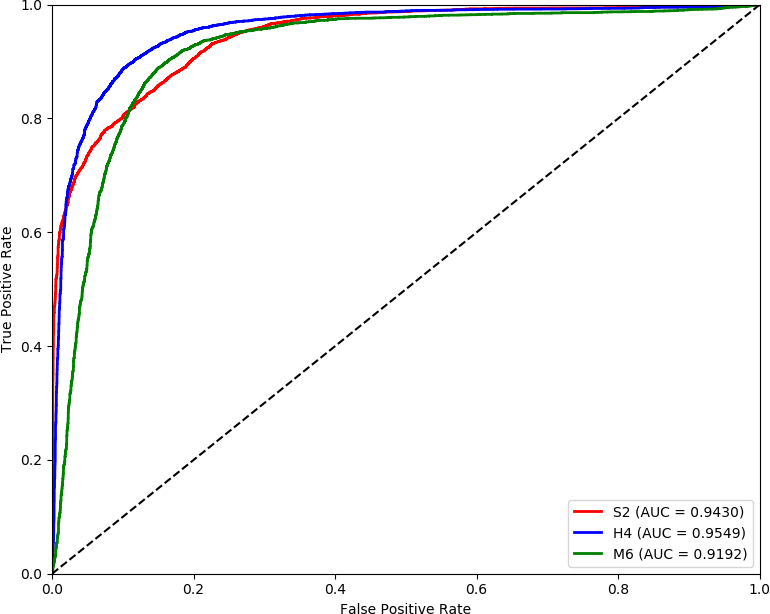
\includegraphics[width=.8\textwidth]{dados/figuras/ROC_H_10_6.png}
 \caption{Curvas ROC dos testes com o cenário H.10.6 para as CNNs treinadas com os conjuntos S2, H4 e M6 (Autoria própria).}
 \label{fig:I_Wanna_ROC!}
\end{figure}

Essa disparidade entre as métricas avaliadas pode ser explicada ao se analisar as matrizes de confusão\footnote{Matriz de confusão é uma tabela que mostra os resultados obtidos por um classificador. As linhas representam os rótulos reais, e as colunas o predito pelo classificador.} dos testes. A Tabela \ref{tab:matrix_reloaded} compara as matrizes de confusão, acurácia, precisão\footnote{Proporção de verdadeiros positivos em relação a todas predições positivas.} e revocação\footnote{Taxa de verdadeiros positivos.} obtidas pelas CNNs treinadas com os conjuntos S2 e H4 quando testados no cenário H.10.6.

\begin{table}[!htb]
\centering
\begin{tabular}{c|c|c|c|c|@{}m{0pt}@{}}
\cline{2-5}
		                          & \textbf{\begin{tabular}[c]{@{}c@{}}Matriz de\\ Confusão\end{tabular}}   & \textbf{Acurácia} & \textbf{Precisão} & \textbf{Revocação} &\\[20pt] \hline
\multicolumn{1}{|c|}{\textbf{H4}} & $\left[ \begin{array}{cc} 4156 & 844 \\ 300 & 4700 \end{array} \right]$ & 88,56\%           & 0.8477            & 0.94               &\\[21pt] \hline
\multicolumn{1}{|c|}{\textbf{S2}} & $\left[ \begin{array}{cc} 2548 & 2452 \\ 62 & 4938 \end{array} \right]$ & 74,86\%           & 0.6682            & 0.9876             &\\[21pt] \hline
\end{tabular}
\caption{Outras métricas dos testes realizados no cenário H.10.6 com as CNNs treinadas com os conjuntos H4 e S2.}
\label{tab:matrix_reloaded}
\end{table}

Também é interessante notar a baixa variação das acurácias para o \textit{payload} de 0.6 bpp, onde se tem um desvio padrão de apenas 0,093. A Tabela \ref{tab:cnn_s2} ilustra os resultados obtidos ao utilizar diferentes cenários de teste.

\begin{table}[!ht]
\centering
\begin{tabular}{c|c|c|c|c|}
\cline{2-5}
\textbf{}                             & \textbf{x = 0.1} & \textbf{x = 0.2} & \textbf{x = 0.4} & \textbf{x = 0.6} \\ \hline
\multicolumn{1}{|c|}{\textbf{H.0.x}}  & 56,1\%           & 67,59\%          & 73,59\%          & 74,76\%          \\ \hline
\multicolumn{1}{|c|}{\textbf{H.10.x}} & \textbf{57,94\%} & \textbf{69,02\%} & \textbf{73,87\%} & \textbf{74,86\%} \\ \hline
\multicolumn{1}{|c|}{\textbf{S.0.x}}  & 53,65\%          & 63,21\%          & 73,09\%          & 74,73\%          \\ \hline
\multicolumn{1}{|c|}{\textbf{S.7.x}}  & 55,03\%          & 66,78\%          & 73,65\%          & 74,83\%          \\ \hline
\multicolumn{1}{|c|}{\textbf{S.10.x}} & 54,69\%          & 65,59\%          & 73,47\%          & 74,76\%          \\ \hline
\multicolumn{1}{|c|}{\textbf{S.12.x}} & 54,3\%           & 65,36\%          & 73,45\%          & 74,79\%          \\ \hline
\multicolumn{1}{|c|}{\textbf{M.-.x}}  & 54,18\%          & 64,17\%          & 72,88\%          & 74,55\%          \\ \hline
\end{tabular}
\caption{Acurácias dos testes da CNN com o conjunto de treinamento S2.}
\label{tab:cnn_s2}
\end{table}

\subsection{Conjunto de Treinamento S4}

Os testes com a CNN treinada neste conjunto apresentaram bons resultados, ficando entre os melhores para \textit{payloads} de 0.1, 0.2 e 0.4 bpp para todos algoritmos. A Tabela \ref{tab:cnn_s4} apresenta as acurácias para todos os cenários de teste.

\begin{table}[!htb]
\centering
\begin{tabular}{c|c|c|c|c|}
\cline{2-5}
\textbf{}                             & \textbf{x = 0.1} & \textbf{x = 0.2} & \textbf{x = 0.4} & \textbf{x = 0.6} \\ \hline
\multicolumn{1}{|c|}{\textbf{H.0.x}}  & 53,78\%          & 66,74\%          & 80,25\%          & 84,43\%          \\ \hline
\multicolumn{1}{|c|}{\textbf{H.10.x}} & \textbf{55,21\%} & \textbf{69,04\%} & \textbf{81,07\%} & 84,50\%          \\ \hline
\multicolumn{1}{|c|}{\textbf{S.0.x}}  & 52,28\%          & 59,95\%          & 79,15\%          & 84,56\%          \\ \hline
\multicolumn{1}{|c|}{\textbf{S.7.x}}  & 53,08\%          & 64,30\%          & 80,94\%          & \textbf{84,89\%} \\ \hline
\multicolumn{1}{|c|}{\textbf{S.10.x}} & 52,82\%          & 62,80\%          & 80,43\%          & 84,77\%          \\ \hline
\multicolumn{1}{|c|}{\textbf{S.12.x}} & 52,64\%          & 62,39\%          & 80,00\%          & 84,65\%          \\ \hline
\multicolumn{1}{|c|}{\textbf{M.-.x}}  & 52,58\%          & 61,82\%          & 78,03\%          & 83,30\%          \\ \hline
\end{tabular}
\caption{Acurácias dos testes da CNN com o conjunto de treinamento S4.}
\label{tab:cnn_s4}
\end{table}


\subsection{Conjunto de Treinamento S6}

Este foi o conjunto de treinamento que obteve a maior acurácia para todos os cenários de teste do algoritmo S-UNIWARD com \textit{payload} de 0.6 bpp. Tendo mostrado também boa acurácia para outros algoritmos com o mesmo \textit{payload}. Porém foi um dos piores nos testes com \textit{payload} de 0.1 bpp, como pode ser visto na Tabela \ref{tab:cnn_s6}.

\begin{table}[!htb]
\centering
\begin{tabular}{c|c|c|c|c|}
\cline{2-5}
\textbf{}                             & \textbf{x = 0.1} & \textbf{x = 0.2} & \textbf{x = 0.4} & \textbf{x = 0.6} \\ \hline
\multicolumn{1}{|c|}{\textbf{H.0.x}}  & 51,12\%          & 59,21\%          & 75,72\%          & 87,01\%          \\ \hline
\multicolumn{1}{|c|}{\textbf{H.10.x}} & \textbf{51,67\%} & \textbf{61,38\%} & 77,58\%          & 87,86\%          \\ \hline
\multicolumn{1}{|c|}{\textbf{S.0.x}}  & 50,68\%          & 55,24\%          & 74,52\%          & 87,24\%          \\ \hline
\multicolumn{1}{|c|}{\textbf{S.7.x}}  & 50,98\%          & 58,51\%          & \textbf{77,67\%} & \textbf{89,12\%} \\ \hline
\multicolumn{1}{|c|}{\textbf{S.10.x}} & 50,72\%          & 57,16\%          & 76,50\%          & 88,37\%          \\ \hline
\multicolumn{1}{|c|}{\textbf{S.12.x}} & 50,81\%          & 56,80\%          & 75,89\%          & 88,12\%          \\ \hline
\multicolumn{1}{|c|}{\textbf{M.-.x}}  & 50,73\%          & 55,52\%          & 72,75\%          & 83,85\%          \\ \hline
\end{tabular}
\caption{Acurácias dos testes da CNN com o conjunto de treinamento S6.}
\label{tab:cnn_s6}
\end{table}


\subsection{Conjunto de Treinamento M1}

Este conjunto, treinado com a base contendo imagens esteganografadas com o algoritmo MiPOD, apresentou resultados medianos em todos os testes. A Tabela \ref{tab:cnn_m1} exibe as acurácias obtidas.

\begin{table}[!htb]
\centering
\begin{tabular}{c|c|c|c|c|}
\cline{2-5}
\textbf{}                             & \textbf{x = 0.1} & \textbf{x = 0.2} & \textbf{x = 0.4} & \textbf{x = 0.6} \\ \hline
\multicolumn{1}{|c|}{\textbf{H.0.x}}  & 52,87\%          & 61,84\%          & 77,76\%          & 83,15\%          \\ \hline
\multicolumn{1}{|c|}{\textbf{H.10.x}} & \textbf{53,80\%} & \textbf{64,64\%} & \textbf{79,00\%} & \textbf{83,56\%} \\ \hline
\multicolumn{1}{|c|}{\textbf{S.0.x}}  & 51,40\%          & 55,88\%          & 74,84\%          & 82,09\%          \\ \hline
\multicolumn{1}{|c|}{\textbf{S.7.x}}  & 51,98\%          & 58,11\%          & 77,29\%          & 83,08\%          \\ \hline
\multicolumn{1}{|c|}{\textbf{S.10.x}} & 51,72\%          & 57,42\%          & 76,28\%          & 82,85\%          \\ \hline
\multicolumn{1}{|c|}{\textbf{S.12.x}} & 51,65\%          & 57,07\%          & 76,02\%          & 82,63\%          \\ \hline
\multicolumn{1}{|c|}{\textbf{M.-.x}}  & 51,98\%          & 58,18\%          & 76,14\%          & 82,20\%          \\ \hline
\end{tabular}
\caption{Acurácias dos testes da CNN com o conjunto de treinamento M1.}
\label{tab:cnn_m1}
\end{table}

\subsection{Conjunto de Treinamento M2}

Assim como o conjunto S4, o M2 também ficou entre os melhores nos testes com \textit{payloads} de 0.1, 0.2, e 0.4 bpp, porém foi um dos piores nos testes com 0.6. A Tabela \ref{tab:cnn_m2} apresenta os resultados obtidos. Assim como na maioria dos testes, cenário H.10.x foi o que apresentou as maiores taxas de acurácia. 

\begin{table}[!htb]
\centering
\begin{tabular}{c|c|c|c|c|}
\cline{2-5}
\textbf{}                             & \textbf{x = 0.1} & \textbf{x = 0.2} & \textbf{x = 0.4} & \textbf{x = 0.6} \\ \hline
\multicolumn{1}{|c|}{\textbf{H.0.x}}  & 53,80\%          & 63,09\%          & 78,96\%          & 82,46\%          \\ \hline
\multicolumn{1}{|c|}{\textbf{H.10.x}} & \textbf{54,94\%} & \textbf{65,94\%} & \textbf{79,93\%} & \textbf{82,59\%} \\ \hline
\multicolumn{1}{|c|}{\textbf{S.0.x}}  & 52,25\%          & 57,86\%          & 75,74\%          & 81,92\%          \\ \hline
\multicolumn{1}{|c|}{\textbf{S.7.x}}  & 52,92\%          & 60,29\%          & 78,40\%          & 82,46\%          \\ \hline
\multicolumn{1}{|c|}{\textbf{S.10.x}} & 52,72\%          & 59,49\%          & 77,58\%          & 82,27\%          \\ \hline
\multicolumn{1}{|c|}{\textbf{S.12.x}} & 52,64\%          & 58,94\%          & 76,90\%          & 82,10\%          \\ \hline
\multicolumn{1}{|c|}{\textbf{M.-.x}}  & 52,94\%          & 60,59\%          & 77,46\%          & 82,00\%          \\ \hline
\end{tabular}
\caption{Acurácias dos testes da CNN com o conjunto de treinamento M2.}
\label{tab:cnn_m2}
\end{table}


\subsection{Conjunto de Treinamento M4}

A Tabela \ref{tab:cnn_m4} apresenta os resultados obtidos com este conjunto de treinamento, que teve boas taxas de acerto nos testes com \textit{payloads} de 0.4 e 0.6 bpp. Foi o melhor desempenho obtido em todos os testes para o cenário M.-.6, onde alcançou 85.94\% de acurácia, superando inclusive a abordagem com SRM + \textit{ensemble of classifiers}.

\begin{table}[!htb]
\centering
\begin{tabular}{c|c|c|c|c|}
\cline{2-5}
\textbf{}                             & \textbf{x = 0.1} & \textbf{x = 0.2} & \textbf{x = 0.4} & \textbf{x = 0.6} \\ \hline
\multicolumn{1}{|c|}{\textbf{H.0.x}}  & 51,61\%          & 57,49\%          & 79,67\%          & 86,44\%          \\ \hline
\multicolumn{1}{|c|}{\textbf{H.10.x}} & \textbf{52,17\%} & \textbf{60,59\%} & \textbf{81,55\%} & \textbf{87,05\%} \\ \hline
\multicolumn{1}{|c|}{\textbf{S.0.x}}  & 51,09\%          & 54,10\%          & 73,14\%          & 85,51\%          \\ \hline
\multicolumn{1}{|c|}{\textbf{S.7.x}}  & 51,36\%          & 55,54\%          & 78,52\%          & 86,48\%          \\ \hline
\multicolumn{1}{|c|}{\textbf{S.10.x}} & 51,28\%          & 54,83\%          & 76,12\%          & 86,25\%          \\ \hline
\multicolumn{1}{|c|}{\textbf{S.12.x}} & 51,24\%          & 54,73\%          & 75,43\%          & 86,08\%          \\ \hline
\multicolumn{1}{|c|}{\textbf{M.-.x}}  & 51,57\%          & 55,77\%          & 77,14\%          & 85,94\%          \\ \hline
\end{tabular}
\caption{Acurácias dos testes da CNN com o conjunto de treinamento M4.}
\label{tab:cnn_m4}
\end{table}

Observe que o desempenho para os \textit{payloads} 0.1 e 0.2 não foi bom, indicando que o treinamento para o \textit{payload} 0.4 deixa o classificador mais habilitado para identificar maiores quantidades de mensagens escondidas. Ao passo que o treinamento realizado com M1 e M2 obtém 64,64\% e 65,94\% de acurácia para o teste com \textit{payload }0.2, respectivamente, para o M4 o valor é de 60,59\%.

\subsection{Conjunto de Treinamento M6}

Os resultados do conjunto M6, mostrados na Tabela \ref{tab:cnn_m6}, foram os piores em comparação com os obtidos pelos outros conjuntos em grande parte dos testes. Apresentando resultados satisfatórios apenas quando testado com \textit{payload} de 0.6 bpp.

\begin{table}[!htb]
\centering
\begin{tabular}{c|c|c|c|c|}
\cline{2-5}
\textbf{}                             & \textbf{x = 0.1} & \textbf{x = 0.2} & \textbf{x = 0.4} & \textbf{x = 0.6} \\ \hline
\multicolumn{1}{|c|}{\textbf{H.0.x}}  & 50,52\%          & 51,86\%          & 65,65\%          & 84,16\%          \\ \hline
\multicolumn{1}{|c|}{\textbf{H.10.x}} & \textbf{50,63\%} & \textbf{52,29\%} & \textbf{69,96\%} & \textbf{86,12\%} \\ \hline
\multicolumn{1}{|c|}{\textbf{S.0.x}}  & 50,37\%          & 51,35\%          & 57,59\%          & 80,20\%          \\ \hline
\multicolumn{1}{|c|}{\textbf{S.7.x}}  & 50,45\%          & 51,63\%          & 61,46\%          & 84,46\%          \\ \hline
\multicolumn{1}{|c|}{\textbf{S.10.x}} & 50,44\%          & 51,59\%          & 59,65\%          & 82,80\%          \\ \hline
\multicolumn{1}{|c|}{\textbf{S.12.x}} & 50,39\%          & 51,60\%          & 59,30\%          & 82,28\%          \\ \hline
\multicolumn{1}{|c|}{\textbf{M.-.x}}  & 50,48\%          & 51,48\%          & 63,61\%          & 83,87\%          \\ \hline
\end{tabular}
\caption{Acurácias dos testes da CNN com o conjunto de treinamento M6.}
\label{tab:cnn_m6}
\end{table}


% \section{Detecção do LSB \textit{Matching}}
% 
% EXPLICAR AQUI PQ FOI USADA (PARA VALIDAÇÃO).
% MENCIONAR ESTADO DA ARTE (SE É VALIDAÇÃO, DEVE ESTAR COMPATÍVEL)!!!
% 
% O LSB-Matching~\citeauthor{lsb_matching_revised} foi implementado em C++ pelos próprios autores desse trabalho segundo as especificações de \citeonline{sharp2001implementation} e \citeonline{lsb_matching_revised}\footnote{Disponível em: \url{https://github.com/yudi-matsuzake/stegim}.}. 
% 
% A Tabela \ref{tab:lsbespecial} mostra os resultados obtidos com cada um dos conjuntos de treinamento, quando testados com o LSB \textit{Matching}. Os resultados, 
%ESSA ARGUMENTAÇÃO NÃO ESTÁ BOA, CONFORME CONVERSAMOS!!!
%apesar de estarem não estado da arte de detecção do LSB \textit{Matching}, porém, nesse caso ele foi utilizado para apenas a validação da rede. Conforme exemplificado na Figura~\ref{fig:comp}, fica claro perceber o motivo desses resultados quando se analisa a diferença de abordagens dos algoritmos adaptativos e não-adaptativos.

% \begin{table}[!htb]
% \centering
% \caption{Acurácias da detecção do LSB \textit{Matching}.}
% \label{tab:lsbespecial}
% \begin{tabular}{c|c|c|c|c|}
% \cline{2-5}
%                                   & \textbf{0.1} & \textbf{0.2} & \textbf{0.4} & \textbf{0.6} \\ \hline
% \multicolumn{1}{|c|}{\textbf{H1}} & 53,93\%        & 65,03\%        & 83,34\%        & 86,86\%        \\ \hline
% \multicolumn{1}{|c|}{\textbf{H2}} & 53,21\%        & 63,47\%        & 86,62\%        & 89,77\%        \\ \hline
% \multicolumn{1}{|c|}{\textbf{H4}} & 54,25\%        & 70,75\%        & 89,94\%        & 91,06\%        \\ \hline
% \multicolumn{1}{|c|}{\textbf{H6}} & 52,79\%        & 68,85\%        & 91,67\%        & \textbf{95,22}\%        \\ \hline
% \multicolumn{1}{|c|}{\textbf{S1}} & 53,67\%        & 66,29\%        & 89,04\%        & 90,64\%        \\ \hline
% \multicolumn{1}{|c|}{\textbf{S2}} & \textbf{60,81}\%        & 73,75\%        & 75,19\%        & 75,37\%        \\ \hline
% \multicolumn{1}{|c|}{\textbf{S4}} & 60,51\%        & \textbf{81,84}\%        & 86,02\%        & 86,3 \%        \\ \hline
% \multicolumn{1}{|c|}{\textbf{S6}} & 57,75\%        & 79,86\%        & \textbf{93,15}\%        & 93,97\%        \\ \hline
% \multicolumn{1}{|c|}{\textbf{M1}} & 55,41\%        & 72,89\%        & 84,38\%        & 85,71\%        \\ \hline
% \multicolumn{1}{|c|}{\textbf{M2}} & 55,88\%        & 73,42\%        & 84,26\%        & 84,91\%        \\ \hline
% \multicolumn{1}{|c|}{\textbf{M4}} & 53,99\%        & 68,46\%        & 87,99\%        & 89,06\%        \\ \hline
% \multicolumn{1}{|c|}{\textbf{M6}} & 51,78\%        & 57,68\%        & 86,62\%        & 92,26\%        \\ \hline
% \end{tabular}
% \end{table}

\section{Análise dos Resultados}

Os experimentos realizados com o uso de SRM e \textit{ensemble} de classificadores revelaram que essa abordagem é inadequada para esteganálise cega, isto é, detectar a presença de uma mensagem oculta sem conhecimento prévio do algoritmo e \textit{payload} utilizados. Os resultados obtidos só foram bons quando o treinamento e teste foi feito com o mesmo algoritmo, e com uma taxa de bits por pixel igual ou parecida.

Já a CNN, apesar de não ter alcançado os mesmos valores de acurácia que o \textit{ensemble} de classificadores em esteganálise direcionada, se mostrou muito mais eficaz para esteganálise cega, especialmente quando treinada com \textit{payloads} de 0.2 e 0.4 bpp. As únicas exceções a isso são as CNNs treinadas com MiPOD e S-UNIWARD com 0.2 bpp quando testadas com \textit{payload} de 0.6 bpp, onde a acurácia obtida foi muito baixa.

Uma das primeiras hipóteses consideradas no início desse trabalho era que os kernels da CNN poderiam se aproximar dos filtros SRM. Porém, isso não pode ser confirmado com os experimentos,  uma vez que os dois detectores se comportam de forma diferente --- a CNN tendo poder de generalização maior enquanto o SRM se mostra mais especializado.

Outro comportamento pertinente ao se usar a CNN foi a obtenção de piores resultados ao se usar os \textit{payloads} de 0.1 bpp e 0.6 bpp para o treinamento. Isso provavelmente ocorre porque quanto mais extremo o \textit{payload}, mais especializada tende a ficar a rede.

É possível notar também que, nos cenários onde foi utilizado o STC, a acurácia dos detectores foi maior, tanto do SRM e \textit{ensemble} de classificadores quanto da CNN.

Como já esperado, o algoritmo com o uso do descritor SRM teve desempenho notável quando se testando com o algoritmo HUGO, principalmente pelo fato de ter sido estruturado para a esteganálise do mesmo. O que acabou sendo surpreendente é que o seu melhor desempenho é muito superior ao da CNN, diferença discrepante com relação ao resultados dos outros algoritmos. Como pode ser observado na Tabela \ref{tab:hugo_comp}, nos cenários H.0.1 e H.10.1  a diferença chegou a um máximo de 10\%.

\begin{table}[h]
\centering
\caption{Comparação entre os melhores resultados para o algoritmo HUGO com uso do SRM e com uso da CNN}
\label{tab:hugo_comp}
\begin{tabular}{|c|c|c|c|c|c|c|c|c|}
\hline
    & H.0.1   & H.0.2   & H.0.4   & H.0.6   & H.10.1  & H.10.2  & H.10.4  & H.10.6  \\ \hline
SRM & 66,23\% & 73,89\% & 84,60\% & 90,46\% & 67,02\% & 75,30\% & 85,43\% & 91,18\% \\ \hline
CNN & 56,10\% & 67,59\% & 80,25\% & 88,01\% & 57,94\% & 69,04\% & 81,55\% & 88,56\% \\ \hline
\end{tabular}
\end{table}

Apesar das acurácias diferirem bastante, principalmente para o algoritmo HUGO, as AUCs para o \textit{payload} de 0.1 bpp não tem um contraste tão evidente, como mostrado na Figura \ref{fig:ROC_H}(a), na qual a CNN chegou, inclusive, a ter a curva superior ao SRM em vários pontos. Esse mesmo comportamento não se repete para o \textit{payload} de 0.6 bpp, como pode ser visto na Figura \ref{fig:ROC_H}(b), onde a curva do SRM é sempre superior a da CNN.

\begin{figure}[!ht]
\centering
	\subfloat[HUGO 0.1]{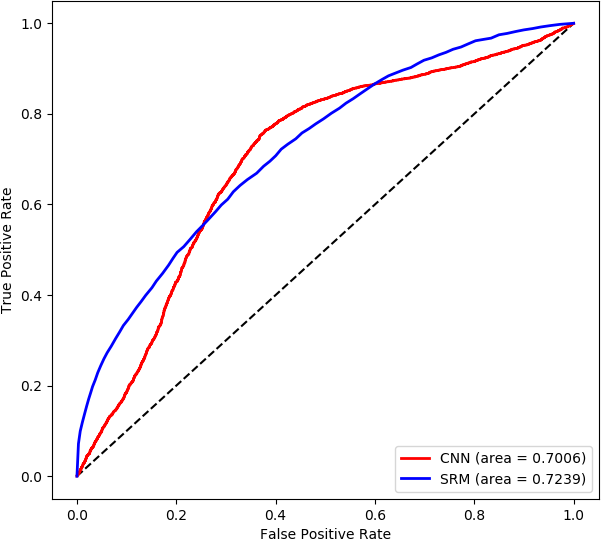
\includegraphics[width=0.45\textwidth]{dados/figuras/H1_H_0_1.png}}\;
	\subfloat[HUGO 0.6]{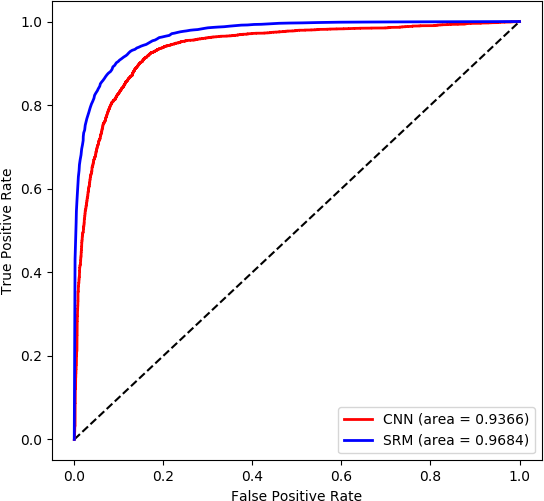
\includegraphics[width=0.45\textwidth]{dados/figuras/H6_H_0_6.png}} 
	\caption{Curvas ROC da CNN e do SRM para os cenários de teste e treino iguais (Autoria própria)}
    \label{fig:ROC_H}
\end{figure}

A Figura \ref{fig:ROC_M} ilustra um conjunto de treino no qual o SRM teve desempenho inferior à CNN em todos os cenários de teste que fazem uso do MiPOD, tanto com relação as acurácias quanto as AUCs. Isso ocorre porque o treino foi feito com um algoritmo de menor complexidade que o de teste, situação que piora consideravelmente a performance do SRM.

\begin{figure}[!htb]
 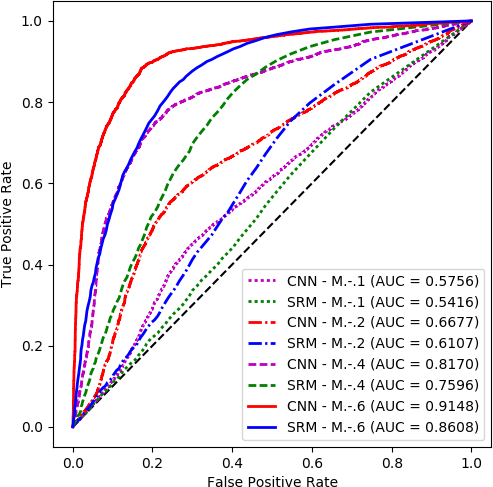
\includegraphics[width=.8\textwidth]{dados/figuras/H6_M-_x.png}
 \caption{Curvas ROC dos testes com o MiPOD e treinos com o cenário H6. (Autoria própria).}
 \label{fig:ROC_M}
\end{figure}

Uma característica em comum às duas arquiteturas foi a maior dificuldade de detectar a presença do algoritmo MiPOD. No caso do SRM, isso é ainda mais notável quando o classificador é treinado com um algoritmo diferente do MiPOD.

Com relação ao desempenho computacional, foi possível notar que o tempo de treino do \textit{ensemble} de classificadores com FLD é muito menor que o da CNN, porém o descritor SRM tem alta complexidade computacional pela quantidade de convoluções que são realizadas para cada filtro do algoritmo. Mesmo com a alta complexidade do descritor, a CNN é mais custosa computacionalmente no processo como um todo. 

Os Apêndices~\ref{chap:apendiceA} e \ref{chap:apendiceB} apresentam os valores de AUC para as duas abordagens.

